\documentclass{article}
\usepackage[utf8]{inputenc}
\usepackage{xcolor}
\usepackage{amsmath}
\usepackage{amssymb}
\usepackage{graphicx}
\usepackage{hyperref}

\title{Neural Networks Exercise Sheet 2}
\author{Pauline Sander s8pasand, Vilém Zouhar vizo00001}

\newcommand{\TODO}[1]{{\color{red} TODO: #1}}
\newcommand{\VV}[1]{{\color{blue} Vilda: #1}}
\newcommand{\PP}[1]{{\color{teal} Pauline: #1}}

\begin{document}

\maketitle

\setcounter{section}{2}
\subsection{Eigenvalue Decomposition \& SVD}

\subsubsection*{a)}
\begin{center}
    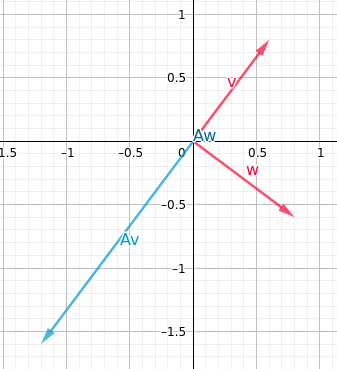
\includegraphics[width=0.5  \linewidth]{img/fig1.png}
\end{center}

The vector $\mathbf{v}$ gets extended and flips its direction, while $\mathbf{w}$ gets projected to zero.

Zero eigenvalue means that there exists a direction which gets lost in this transformation. Formally it means that the transformation has a nontrivial kernel. 

\subsubsection*{b)}

There are infinitely many such vectors: $\{r\cdot \mathbf{v} | r \in \mathbb{R} \backslash \{0\}\}$. Assuming $\mathbf{v}$ is an eigenvectorof $\mathbf{A}$ and $a$ its corresponding eigenvalue, then the following holds: $\mathbf{A} \mathbf{v} = a \cdot \mathbf{v}$, which means that also $\mathbf{A} (r \cdot \mathbf{v}) = a \cdot (r \cdot \mathbf{v})$, which proves that $r \cdot \mathbf{v}$ is also an eigenvector for $\mathbf{A}, r \in \mathbb{R} \backslash \{0\}$.

A specific example: $v' = [0.3, 0.4]^T$

\pagebreak

\subsubsection*{c)}

Straight from the spectral decomposition theorem:

\begin{align*}
    A &= Q \times \Lambda \times Q^{-1} \\
    &=
    \begin{pmatrix}
        0.6 & 0.8 \\
        0.8 & -0.6
    \end{pmatrix}
    \times
    \begin{pmatrix}
        -2 & 0\\
        0 & 0
    \end{pmatrix}
    \times
    \begin{pmatrix}
        0.6 & 0.8\\
        0.8 & -0.6
    \end{pmatrix} \\
    &=
    \begin{pmatrix}
        0.6 & 0.8 \\
        0.8 & -0.6
    \end{pmatrix}
    \times
    \begin{pmatrix}
        -2*0.6 & -2*0.8\\
        0 & 0
    \end{pmatrix}\\
    &=
    \begin{pmatrix}
        -2*0.6*0.6 & -2*0.6*0.8 \\
        -2*0.8*0.6 & -2*0.8*0.8
    \end{pmatrix}
    =
    \begin{pmatrix}
        -0.72 & -0.96 \\
        -0.96 & -1.28
    \end{pmatrix}
\end{align*}

\subsubsection*{d)}

The matrix with columns of eigenvectors, $\mathbf{Q}$, is quaranteed to be orthogonal, because we operate on $\mathbb{R}$. That is why $\mathbf{Q}^T = \mathbf {Q}^{-1}$. Since it is already symmetric, then $\mathbf{Q} = \mathbf{Q}^{-1}$.

\subsubsection*{e)}

\textit{positive definite}: all eigenvalues are $>0$ \\
\textit{positive semidefinite}: all eigenvalues are $\geq0$\\
\textit{negative definite}: all eigenvalues are $<0$ \\
\textit{negative semidefinite}: all eigenvalues are $\leq0$, applies to $\mathbf{A}$ \\
\textit{singular}: a matrix that does not have an inverse ($\text{det}\ \mathbf{M} = 0$), applies to $\mathbf{A}$, since it has a non-trivial kernel

\subsubsection*{f)}

Eigenvalue decomposition requires the matrix to be a square matrix, while SVD can be performed on matrix of any dimensions. Eigenvalue decomposition is then just a specific example of SVD for transformation which preserve the space dimensions.

Furthermore, in case the input matrix is not a symmetric one, the eigenvalue decomposition products will contain complex numbers, which is sometimes undesriable. This does not happen with singular value decomposition.

\subsection{Principal Component Analysis}

\subsubsection*{a)}

\begin{center}
    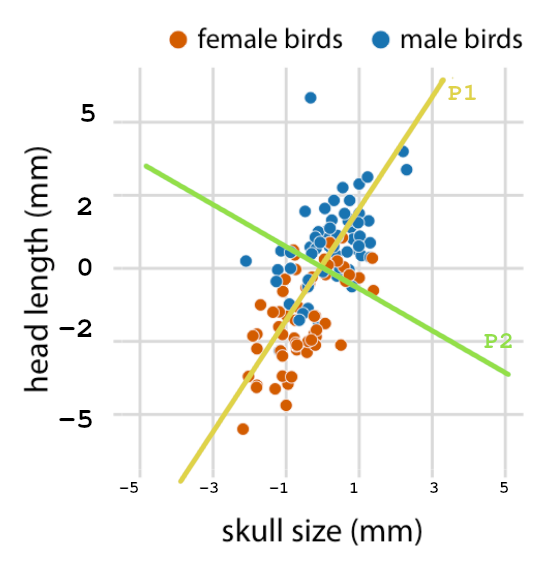
\includegraphics[width=0.75\linewidth]{img/fig2_centered.png}
\end{center}

The data need to average to zero so that the principal components can rotate around the origin.

\subsubsection*{b)}

\begin{center}
    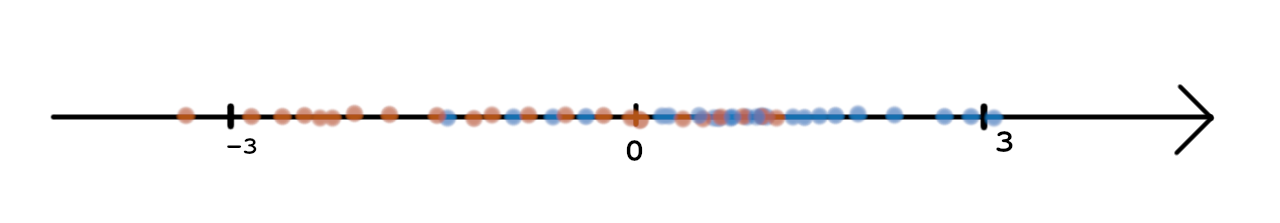
\includegraphics[width=0.85\linewidth]{img/fig3_new.png}
\end{center}


We remove the principal component which contributes less to the explanation of the variance in the data (P2, represented in green in a). We then project all the data points to the remaining component (P1). Mathematically speaking: To calculate the encoding matrix we (1) calculate the covariance matrix of the dataset; (2) calculate the eigenvectors and eigenvalues of that covariance matrix; (3) discard the eigenvector which corresponds to the lower eigenvalue (replace by zeroes); (4) the remaining matrix is the encoding matrix.

\subsubsection*{c)}

\begin{center}
    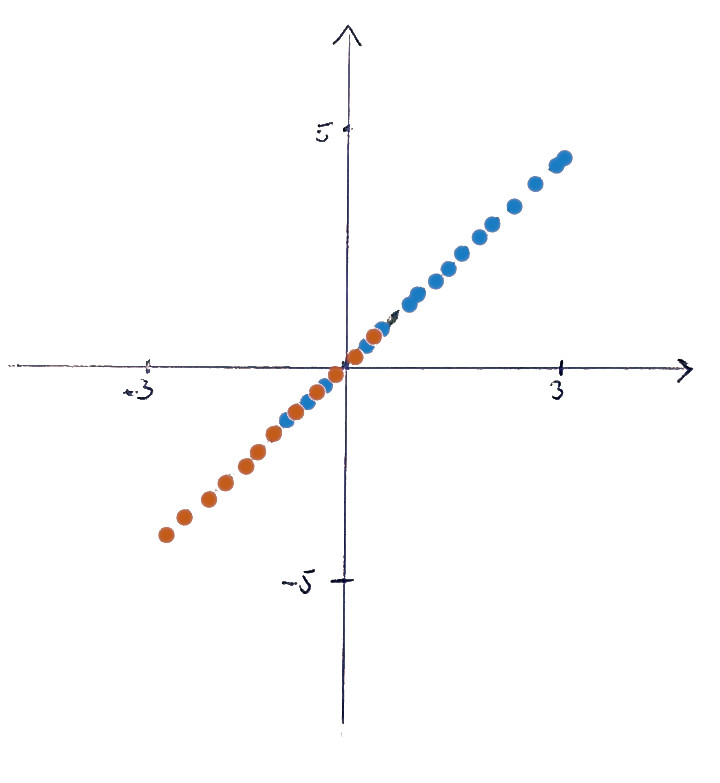
\includegraphics[width=0.75\linewidth]{img/fig3_decoded_new.jpg}
\end{center}

The decoding matrix is the transpose of the encoding matrix.

\subsubsection*{d)}

This dataset could be for example measurement of the position of two kinds of particles from some physics gizmo.
PCA performs badly for this dataset because both principal components account for an equal amount of possible variance. As can be seen in the second plot, a separation of red and blue is not possible when reduced to one component.
\begin{center}
    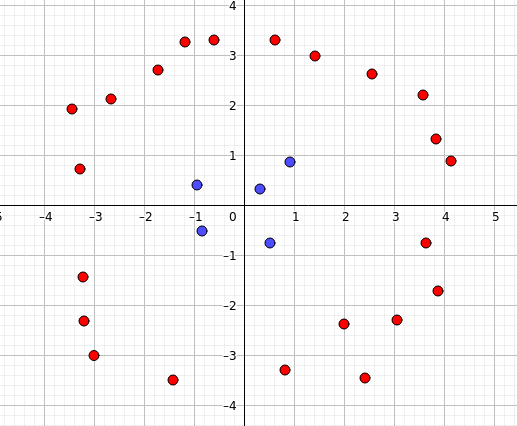
\includegraphics[width=0.85\linewidth]{img/fig4.png}
    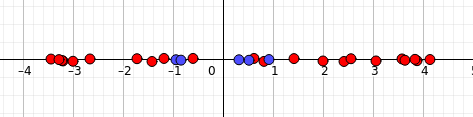
\includegraphics[width=0.85\linewidth]{img/fig4_squeezed.png}
\end{center}

\subsection{Applications}

\subsubsection{Parameter initialization}

Neural networks are known to be susceptible to parameter initialization. With repeated application of the same linear operation, the features could either (1) explode dramatically or (2) shrink to zero, resulting in a very different predicion with just a slight change in the output. This is based on the eigenvalue properties of the matrix which is being applied. It is desired to attempt to preserve the norm of any random vector. If we rescale the whole matrix so that the eigenvalues are around one, this fixes the issue. \href{http://www.d2l.ai/chapter\_appendix-mathematics-for-deep-learning/eigendecomposition.html}{Source: \emph{d2l.ai}}.

\subsubsection{PageRank Algorithm}

This algorithm is used by search engines (Google) to determine the rank of a page and hereby find the perfect ordering of the pages. The importance of a page is calculated only using the links between pages. The eigendecomposition is used to calculate a transition matrix to predict the next ``destinations" of a person surfing the internet. \href{http://www.suchmaschinen-doktor.de/algorithmen/pagerank.html}{Source: \emph{suchmaschinen-doktor}}



\end{document}
